\documentclass[../differential_geometry.tex]{subfiles}
\begin{document}
\section{Aula 12 - 21 de Maio, 2026}
\subsection{Motivações}
\begin{itemize}
	\item Aplicações Suaves entre Superfícies;
	\item Aplicação de Gauss;
	\item A Derivada de uma Aplicação Suave.
\end{itemize}
\subsection{Aplicações Suaves entre Superfícies}
Pedimos que \(f:V\subseteq \mathbb{R}^{n}\rightarrow \mathbb{R}^{m}\) seja uma aplicação suave em um aberto V de \(\mathbb{R}^{n}\), ou seja, que se \(f(x_1, \dotsc , x_{n}) = (f^{1}(x_1, \dotsc , x_{n}), \dotsc , f^{m}(x_1, \dotsc , x_{n}))\), então todas as derivadas parciais das funções \(f^{i}, \; i =1, \dotsc , m\), de todas as ordens, existem e são todas contínuas em V.

Considere a aplicação \(f:S\rightarrow \mathbb{R}\) com \(f(p) = \langle p, p \rangle\), onde S é um cilindro em \(\mathbb{R}^{3}\)
\begin{figure}[H]
	\begin{center}
		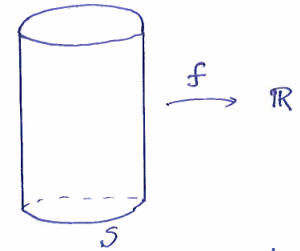
\includegraphics[height=0.5\textheight, width=0.5\textwidth, keepaspectratio]{./Images/smooth_cylinder_12.png}
	\end{center}
\end{figure}
Observe que S não é um aberto de \(\mathbb{R}^{3}\), e que então precisamos definir o significado de suavidade de f neste contexto mais geral.

\begin{def*}
	Seja S uma superfície em \(\mathbb{R}^{n}\). Diremos que uma aplicação \(f:S\rightarrow \mathbb{R}^{m}\) é \textbf{suave no ponto p} se:
	\begin{itemize}
		\item[i)] A composta \(f\circ \underline{x}:U\subseteq \mathbb{R}^{2}\rightarrow \mathbb{R}^{m}\) é suave no ponto q; e
		\item[ii)] A parametrização local \(\underline{x}:U \subseteq \mathbb{R}^{2}\rightarrow S \subseteq \mathbb{R}^{n}\) de S mapeia o ponto q em p, i.e., \(\underline{x}(q) = p\).
	\end{itemize}
	Diremos que \textbf{f é suave em S} se ela for suave em todo ponto p de S.
\end{def*}
Observe que a definição \textbf{não depende} da parametrização local de S:
\begin{figure}[H]
	\begin{center}
		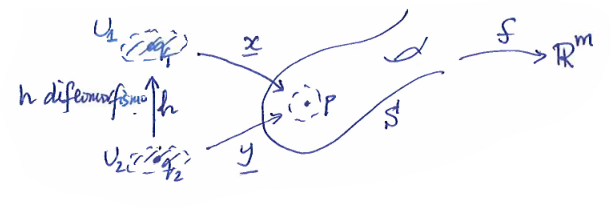
\includegraphics[height=\textheight, width=\textwidth, keepaspectratio]{./Images/smooth_function_12.png}
	\end{center}
	\caption{a composta \(f\circ \underline{x}\) será suave se, e somente se, \(f\circ y = f\circ (\underline{x}\circ h) = (f\circ \underline{x})\circ h\) for suave. }
\end{figure}
\begin{example}[Cilindro]
	Para o caso do cilindro que estávamos vendo ao início, ele é dado por
	\[
		x^{2} + y^{2} = 1.
	\]
	Uma de suas parametrizações locais é da forma
	\[
		\underline{x}(\theta , z) = (\cos^{}{(\theta )}, \sin^{}{(\theta )}, z), \quad (\theta , z)\in \mathbb{R}^{2}.
	\]
	Seja \(f:S\rightarrow \mathbb{R}\) dada por \(f(p) = \langle p, p \rangle\); então, temos
	\[
		f(\underline{x}(\theta , z)) = \langle (\cos^{}{\theta }, \sin^{}{\theta }, z), (\cos^{}{\theta }, \sin^{}{\theta }, z) \rangle = 1 + z^{2},
	\]
	que é uma função suave. Portanto, f é suave.
\end{example}

\pagebreak
\subsection{Aplicação de Gauss}
A aplicação de Gauss tem por ideia associar a cada ponto p e m uma superfície S um vetor normal unitário a S neste ponto:
\begin{figure}[H]
	\begin{center}
		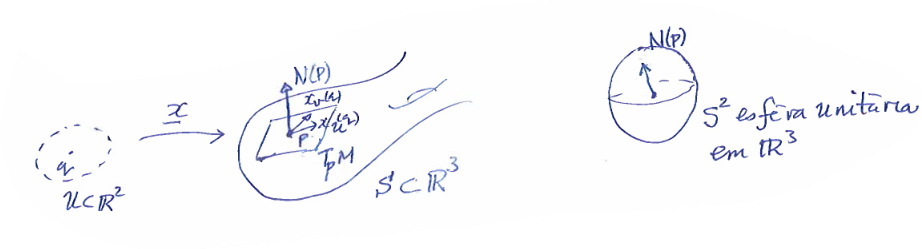
\includegraphics[height=\textheight, width=\textwidth, keepaspectratio]{./Images/gauss_application_12.png}
	\end{center}
\end{figure}
\begin{def*}
	Seja \(\underline{x}:U \subseteq \mathbb{R}^{2}\rightarrow S \subseteq \mathbb{R}^{3}\) uma parametrização local de s. A \textbf{aplicação de Gauss N} é dada por
	\[
		N(\underline{x}(u, v)) = \frac{\underline{x}_{u}\times \underline{x}_{v}(u, v)}{\Vert \underline{x}_{u} \times \underline{x}_{v} \Vert}. \; \square
	\]
\end{def*}
Note que a aplicação \(N\circ \underline{x}:U\subseteq \mathbb{R}^{2}\rightarrow \mathbb{R}^{3}\) é uma aplicação suave!

\begin{tcolorbox}[
		skin=enhanced,
		title=Observação,
		fonttitle=\bfseries,
		colframe=black,
		colbacktitle=cyan!75!white,
		colback=cyan!15,
		colbacklower=black,
		coltitle=black,
		drop fuzzy shadow,
		%drop large lifted shadow
	]
	A aplicação de Gauss é bem-definida em \(\underline{x}(U) \subseteq S\), mas nem sempre ela é bem-definida em toda S; por exemplo, basta considerar o caso da faixa de Möbius, que tem dois vetores normais distintos num mesmo ponto:
	\begin{figure}[H]
		\begin{center}
			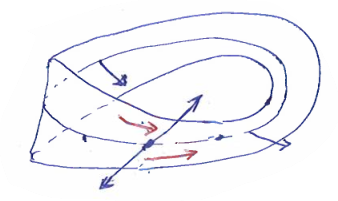
\includegraphics[height=\textheight, width=\textwidth, keepaspectratio]{./Images/mobius_strip_12.png}
		\end{center}
	\end{figure}
	Ela até rasgou a cor pra fora da observação!
\end{tcolorbox}
\begin{example}[Gráfico de Função Suave]
	Como primeiro exemplo, vamos tomar o gráfico da função suave g:
	\[
		S = \{(u, v, g(u, v)):\; (u, v)\in U \subseteq \mathbb{R}^2\}.
	\]
	Temos, aqui,
	\[
		\underline{x}(u, v) = (u, v, g(u, v)) \Rightarrow \underline{x}_{u}(u, v) = (1, 0, g_{u}(u, v)) \;\& \; \underline{x}_{v}(u, v) = (0, 1, g_{v}(u, v)).
	\]
	Portanto, num ponto qualquer do gráfico da função g, o vetor normal é
	\[
		N(\underline{x}(u, v)) = \frac{(-g_{u}(u, v), -g_{v}(u, v), 1)}{\sqrt[]{1+g_{u}^{2}(u, v) + g_{v}^{2}(u, v)}}.
	\]
\end{example}
\begin{example}[Catenoide]
	Para a catenoide, usaremos a parametrização
	\[
		\underline{x}(u, v) = (\cosh^{}{v}\cos^{}{u}, \cosh^{}{v}\sin^{}{u}, v),
	\]
	resultando nas derivadas
	\begin{align*}
		 & \underline{x}_{u}(u, v) = (-\cosh^{}{v}\sin^{}{u}, \cosh^{}{v}\cos^{}{u}, 0) \\
		 & \underline{x}_{v}(u, v) = (\sinh^{}{v}\cos^{}{u}, \sinh^{}{v}\sin^{}{u}, 1).
	\end{align*}
	Logo,
	\[
		N(\underline{x}(u, v)) = \frac{1}{\cosh^{}{v}}(\cos^{}{u}, \sin^{}{u}, -\sinh^{}{v}).
	\]
\end{example}
\begin{example}[Esfera]
	Vamos considerar a esfera dada por
	\[
		S = S^{2}:\; x^{2} + y^{2} + z^{2} = 1.
	\]
	Tome \(f(x, y, z) = x^{2} + y^{2} + z^{2}-1\), tal que \(S = f^{-1}(0)\). Um vetor normal a S no ponto \((x, y, z)\in S\) é, então,
	\[
		\nabla f(x, y, z) = (2x, 2y, 2z).
	\]
	Daí, como \(\Vert \nabla f(x, y, z) \Vert=2\), obtemos
	\[
		N(x, y, z) = \frac{\nabla f}{\Vert \nabla f \Vert}(x, y, z) = (x, y, z),
	\]
	ou seja, a aplicação de Gauss é a identidade!
	\begin{figure}[H]
		\begin{center}
			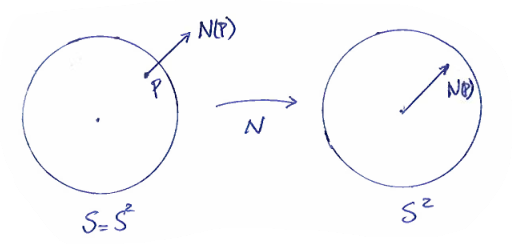
\includegraphics[height=0.6\textheight, width=0.6\textwidth, keepaspectratio]{./Images/derivative_of_gauss_12.png}
		\end{center}
	\end{figure}
\end{example}

\subsection{A Derivada de uma Aplicação Suave}
\begin{def*}
	Seja S uma superfície suave e \(f:S\rightarrow \mathbb{R}^{m}\) uma aplicação suave. A \textbf{derivada de f em um ponto p} de S é a aplicação linear
	\[
		\mathrm{d}f_{p}:T_{p}S\rightarrow \mathbb{R}^{m}
	\]
	tal que
	\[
		\mathrm{d}f_{p}(\underline{x}_{u}(q)) = \frac{\partial^{}}{\partial u^{}}(f\circ \underline{x})(q) \quad\&\quad \mathrm{d}f_{p}(\underline{x}_{u}(q)) = \frac{\partial^{}}{\partial v^{}}(f\circ \underline{x})(q),
	\]
	onde \(\underline{x}:U\subseteq \mathbb{R}^{2}\rightarrow S \subseteq \mathbb{R}^{n}\) é uma parametrização local de S com \(\underline{x}(q) = p.\; \square\)
\end{def*}

Como \(\{\underline{x}_{u}(q), \underline{x}_{v}(q)\}\) é uma base de \(T_{p}S\), a derivada \(\mathrm{d}f_{p}\) é definida em todo \(T_{p}S\), bastando utilizar a linearidade para obter os casos gerais:
\[
	\mathrm{d}f_{p}(a\underline{x}_{u}(q) + b\underline{x}_{v}(q)) = a \mathrm{d}f_{p}(\underline{x}_{u}(q)) + b \mathrm{d}f_{p}(\underline{x}_{v}(q)).
\]

No entanto, precisamos mostrar que \(\mathrm{d}f_{p}\) não depende da parametrização local de S. Com efeito, sabemos que \(T_{p}S\) é o conjunto dos vetores tangentes a S em p; seja, então, \(\alpha :(-\varepsilon , \varepsilon )\rightarrow S\) uma curva em S com \(\alpha (0) = p = \underline{x}(q)\) e suponha que \(\alpha (t) = \underline{x}(u(t), v(t))\).
Com isso,
\[
	\alpha '(0) = u'(0)\underline{x}_{u}(q) + v'(0)\underline{x}_{v}(q),
\]
e obtemos duas coisas: a primeira é
\[
	(f\circ \alpha )(t) = f(\underline{x}(u(t), v(t))) = (f\circ \underline{x})(u(t), v(t))
\]
e a segunda é que
\begin{align*}
	(f\circ \alpha )'(0) & = u'(0)\mathrm{d}f_{p}(\underline{x}_{u}(q)) + v'(0) \frac{\partial^{}}{\partial v^{}}(f\circ \underline{x})(q) \\
	                     & = u'(0) \mathrm{d}f_{p}(\underline{x}_{u}(q)) + v'(0) \mathrm{d}f_{p}(\underline{x}_{v}(q))                     \\
	                     & = \mathrm{d}f_{p}(u'(0)\underline{x}_{u}(q) + v'(0) \underline{x}_{v}(q))                                       \\
	                     & = \mathrm{d}f_{p}(\alpha'(0)),
\end{align*}
provando que \(\mathrm{d}f_{p}\) não depende da parametrização local de S em p.
\begin{figure}[H]
	\begin{center}
		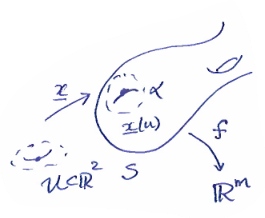
\includegraphics[height=0.5\textheight, width=0.5\textwidth, keepaspectratio]{./Images/parametrization_independence_12.png}
	\end{center}
\end{figure}

Adiante, utilizaremos as seguintes notações:
\begin{align*}
	 & \tikz[baseline=-0.5ex]\draw[black, fill=black, radius=1.5pt](0, 0)circle;\; \mathrm{d}f_{p}:T_{p}S\rightarrow \mathbb{R}^{m}                                                       \\
	 & \tikz[baseline=-0.5ex]\draw[black, fill=black, radius=1.5pt](0, 0)circle;\; f_{u} = \mathrm{d}f_{p}(\underline{x}_u) = \frac{\partial^{}}{\partial u^{}}(f\circ \underline{x})     \\
	 & \tikz[baseline=-0.5ex]\draw[black, fill=black, radius=1.5pt](0, 0)circle;\; f_{v} = \mathrm{d}f_{p}(\underline{x}_{v}) = \frac{\partial^{}f}{\partial v^{}}(f\circ \underline{x}).
\end{align*}

\begin{example}[Esfera]
	Seja S um cilindro em \(\mathbb{R}^{3}\) de equação \(x^{2} + y^{2} = 1\) e
	\[
		f:S\rightarrow \mathbb{R},\; f(p) = \langle p, p \rangle.
	\]
	Anteriormente, vimos que
	\[
		f(\underline{x}(\theta , z)) = 1 + z^{2};
	\]
	logo,
	\[
		f_{\theta } = 0 \quad\&\quad f_{z} = 2z.
	\]
\end{example}
\begin{example}[Catenoide]
	A aplicação de Gauss da Catenoide, como vimos, é
	\[
		N(\underline{x}(u, v)) = \frac{1}{\cosh^{}{v}}(\cos^{}{u}, \sin^{}{u}, - \sinh^{}{v}).
	\]
	Logo,
	\[
		N_{u}=\frac{1}{\cosh^{}{v}}(-\sin^{}{u}, \cos^{}{u}, 0)
	\]
	e
	\[
		N_{v}=\frac{1}{\cosh^{2}{v}}(-\cos^{}{u}\sinh^{}{v}, -\sin^{}{u}\sinh^{}{v}, -1).
	\]
\end{example}

Agora, seja \(f:S\rightarrow \mathbb{R}^{m}\) uma aplicação suave e suponha que \(f(S)\subseteq \tilde{S}\), onde \(\tilde{S}\) é uma superfície em \(\mathbb{R}^{m}\). Temos, para p em S, \(\mathrm{d}f_{p}:T_{p}S\rightarrow \mathbb{R}^{m}\), e vimos que
\[
	\mathrm{d}f_{p}(\alpha '(0))=(f\circ \alpha )'(0),
\]
onde \(\alpha :(-\varepsilon , \varepsilon )\rightarrow S\) é uma curva em S com \(\alpha (0) = p\). Logo, \(\mathrm{d}f_{p}(\alpha '(0))\) é um vetor tangente a \(\tilde{S}\) no ponto \(f(p)\), pois \(f\circ \alpha :(-\varepsilon , \varepsilon )\rightarrow \tilde{S}\) é uma curva em \(\tilde{S}\) com
\[
	(f\circ \alpha )(0) = f(p),
\]
do que segue que \(\mathrm{d}f_{p}\) é uma aplicação do tipo
\[
	\mathrm{d}f_{p}:T_{p}S\rightarrow T_{f(p)}\tilde{S}.
\]
Para a aplicação de Gauss de uma superfície S contida em \(\mathbb{R}^{3}\), \(N:S\rightarrow S^{2}\subseteq \mathbb{R}^{3}\), então
\[
	\mathrm{d}N_{p}:T_{p}S\rightarrow T_{N(p)}S^{2} = T_{p}S,
\]
ou seja, a derivada da aplicação de Gauss
\[
	\mathrm{d}N_{p}:T_{p}S\rightarrow T_{p}S
\]
é um operador linear!
\begin{figure}[H]
	\begin{center}
		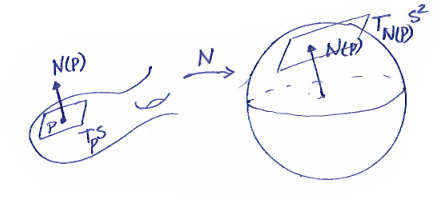
\includegraphics[height=0.7\textheight, width=0.7\textwidth, keepaspectratio]{./Images/gauss_spheres_12.png}
	\end{center}
\end{figure}


\end{document}

